\section{持久连接和管道}
\subsection{概述}
\ \\
通常http客户端发出请求后即关闭连接。这样每次请求或响应均需重新建立连接,造成资源浪费。http持久连接指客户端发出请求、服务器完成响应后也不直接关闭连接,而是等待一段时间后再关闭,这样可以节约资源。持久连接的HTTP报文须增加Connection: Keep-Alive字段。HTTP 1.1默认使用持久连接。

http管道(pipeline)指客户端无需等待服务器响应即可同时发送多个请求,即可以在一个TCP报文发送多个请求。该技术可以减少TCP报文的发送次数,提升资源使用率。
\subsection{实现}
\ \\
对于持久连接,我们在响应头增加Connection: Keep-Alive字段,实现持久连接。

对于http管道,我们将服务器收到的报文按内容拆分为多个http请求,并按序进行处理,向客户端返回结果。
\subsection{测试}
为测试http管道,我们首先开启浏览器的管线化选项。为触发浏览器的管线化请求,我们实现了一个网页,路径为/img,用来展示上传文件中所有的图片。加载该网页须下载多个图片文件,支持管线化的浏览器会将这多个下载请求使用管线化技术发送。图\ref{pipeline}表明该网页能够正常加载所有图片,表明我们的服务端能良好支持管线化请求。

\begin{figure}
\begin{center}
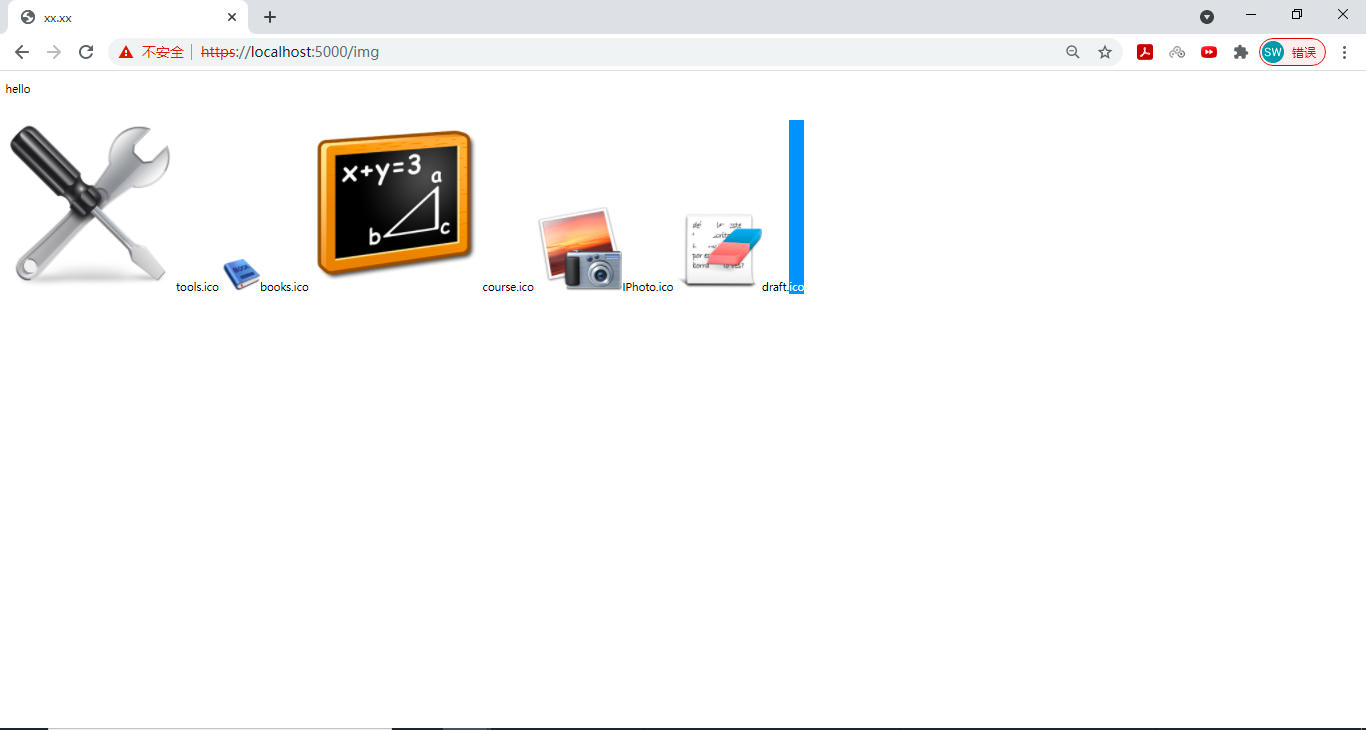
\includegraphics[width=\textwidth]{figs/pipeline.PNG}
\end{center}
\caption{管线化}
\label{pipeline}
\end{figure}